\documentclass[aspectratio=169]{beamer}
\setbeamertemplate{navigation symbols}{}
\usepackage{graphicx}
\usepackage{stmaryrd}
\usepackage[T1,T2A]{fontenc}
\usepackage[utf8]{inputenc}
\usepackage[english,russian]{babel}
\usepackage{amsmath}
\usepackage{amsfonts}
\usepackage{amssymb}
\usepackage{makeidx}
\usepackage{verbatim}
\usepackage{amsthm}
\usepackage{bnf}
\usepackage{tikz}
\usepackage{enumerate}
\usepackage{mathtext}
\usepackage{mathtools}
\usepackage{mathabx}
%\usepackage[left=2cm,right=2cm,top=2cm,bottom=2cm,bindingoffset=0cm]{geometry}
\usepackage{proof}
%\usepackage{paracol}
%\usepackage{enumitem}
\usepackage{color}
\usepackage{colortbl}
%\usepackage{minted}
%\usepackage{hyperref}
\usetikzlibrary{graphs}
\usetikzlibrary{graphs.standard}
\usetikzlibrary{automata,positioning}
\usepackage{float}

\begin{document}

%\theoremstyle{dfn}
\newtheorem{dfn}{Определение}[section]
\newtheorem{nte}{Замечание}[section]

\newtheorem{axiom}{Аксиома}[section]
\newtheorem{thm}{Теорема}[section]
\newtheorem{lmm}[theorem]{Лемма}
\newtheorem{statement}{Утверждение}[section]
\newtheorem{oun_paragraph}{Пункт}[section]
\newtheorem{cons}{Следствие}[section]
\newtheorem*{exm}{Пример}

\newcommand{\comb}[1]{\operatorname{\bf{\textrm{#1}}}}
\newcommand{\func}[1]{\operatorname{#1}}
\newcommand{\reduction}[1]{{\color{OrangeRed}#1}}
\newcommand{\set}[1]{\left\{#1\right\}}

\def\from#1{\par \parbox{0.7\textwidth}{\par \hfill\raggedleft \it #1}} 

\begin{frame}{}
\begin{center}\Large Лекция 5.\\ \Large Обобщённая типовая система, лямбда-куб\end{center}
\end{frame}

\begin{frame}[fragile]{Генерики, зависимые типы}

%Рассмотрим код:

\begin{verbatim}
template <class X>
class Z {
    X field;
}
\end{verbatim}

Что такое $Z$? Это функция, возвращающая тип по другому типу (генерик). %$Z : \star\rightarrow\star$

\begin{verbatim}
int main() {
    unsigned sz;
    std::cin >> sz;
    int temp_array [sz];
    std::cout << sizeof(temp_array);
    return 0;
}
\end{verbatim}

Что такое конструкция \verb!int[sz]!? Это функция, возвращающая тип по значению (зависимый тип).

\end{frame}

\begin{frame}{Терминология: типы, рода, сорта}

Мы будем рассматривать конструкции следующих сортов:
\vspace{0.3cm}\begin{tabular}{lll}
Название сорта & Примеры сортов & Примеры конструкций, имеющих сорт\\\hline
Тип & $\alpha$, $\alpha\rightarrow\beta$, $\star\rightarrow\alpha$ & $3:\texttt{int}, \texttt{id}: \forall\alpha.\alpha\rightarrow\alpha$\\
Род (kind) & $\star$, $\star\rightarrow\star$, $\alpha\rightarrow\star$ & $\texttt{list}: \star\rightarrow\star$\\
Сорт & $\openbox$ & $\star\rightarrow\star : \openbox$
\end{tabular}

\end{frame}

\begin{frame}{Язык обобщённой типовой системы}

Откажемся от различных пространств имён для значений, типов и прочего, 
а также от синтаксического их разделения. Все переменные для значений
любого сорта, все лямбда-выражения для любых функций --- всё записывается
единообразно.

\begin{dfn}[cинтаксис выражений]
Константы сортов: $c ::= \{\star,\openbox\}$

Выражение:
$$T ::= x \mid c \mid T\ T \mid \lambda x^T.\ T \mid \Pi x^T.\ T$$\vspace{-0.5cm}

Сокращения:
$$A \rightarrow B ::= \Pi x^A.B,\quad x \notin FV(B)$$
$$\forall x.P ::= \Pi x^\star.P\quad\Lambda x.\sigma ::= \lambda x^\star.\sigma$$

Метапеременные термов: $A,B,C,\dots,\quad \rho,\sigma,\tau,\dots$. \\
Метапеременные переменных: $x,y,z$
\end{dfn}


\end{frame}

\begin{frame}{Что такое $\Pi$}

Неформально: $\Pi$ --- аналог лямбда-выражения для типизации конструкции: $$\lambda x^\tau.P : \Pi x^\tau.\pi$$

Вспомним сокращения:
$$A \rightarrow B ::= \Pi x^A.B,\ x \notin FV(B)\qquad\forall x.P ::= \Pi x^\star.P$$

И рассмотрим map:
$$\texttt{map} : \forall a.\forall b.(a \rightarrow b) \rightarrow [a]  \rightarrow[b]$$

Перепишем:
$$\texttt{map} : \Pi a^\star.\Pi b^\star.(\Pi f^{\Pi x^a.b}.\Pi l^{[a]}.[b])$$

Заметим, что операция $[\sigma]$ строит из $\sigma$ другой тип, то есть
$[\sigma] = (\lambda x^\star.\langle\text{тип реализации списка из }x\rangle) \sigma$, можем раскрыть дальше:
$$\texttt{map} : \Pi a^\star.\Pi b^\star.(\Pi f^{\Pi x^a.b}.\Pi l^{(\lambda x^\star\dots) a}.(\lambda x^\star\dots)b)$$

Заметим, что $\lambda \sigma^\star.[\sigma] : \star\rightarrow\star$

\end{frame}

\begin{frame}{Обобщённая типовая система: семейство систем}

Семейство параметризовано множеством пар $\mathcal{S}\subseteq\{\star,\openbox\}\times\{\star,\openbox\}$\\
Аксиома:
    $$\infer{\vdash \star : \openbox}{}$$

Общие правила вывода: $\sigma \in \{\star,\openbox\}$
    $$\infer[x \not \in \Gamma]{\Gamma, x : A \vdash x : A}{\Gamma \vdash A:\sigma}\quad\quad\infer{\Gamma, x : C \vdash A:B}{\Gamma \vdash A:B \qquad \Gamma \vdash C:\sigma}$$
    $$\infer{\Gamma \vdash A:B'}{\Gamma \vdash A:B \qquad \Gamma \vdash B':\sigma \qquad B =_\beta B'}\quad\quad\infer{\Gamma \vdash (F\ H) : B[x := H]}{\Gamma \vdash F : (\Pi x^A.B) \qquad \Gamma \vdash H : A}$$

Частные правила: $\langle \sigma_1, \sigma_2 \rangle \in \mathcal{S}$

    $$\infer[\Pi\text{-правило}]{\Gamma \vdash (\Pi x^A.B) : \sigma_2}{\Gamma \vdash A : \sigma_1 \qquad \Gamma, x : A \vdash B : \sigma_2}$$
    $$\infer[\lambda\text{-правило}]{\Gamma \vdash (\lambda x^A . P) : (\Pi x^A. B)}{\Gamma \vdash A:\sigma_1 \qquad \Gamma, x : A \vdash P : B \qquad \Gamma, x : A \vdash B : \sigma_2}$$

\end{frame}

\begin{frame}{Типизация $\Lambda \alpha.\lambda x^\alpha.x$}
Выражение $\Lambda \alpha.\lambda x^\alpha.x$ перепишется как $\lambda \alpha^\star.\lambda x^\alpha.x$, ожидаем тип
$\Pi \alpha^\star.\Pi x^\alpha.\alpha$.

Потребуются частные правила для $\langle\star,\star\rangle$ и $\langle\openbox,\star\rangle$.
    $$\infer{\Gamma \vdash (\Pi x^A.B) : \sigma_2}{\Gamma \vdash A : \sigma_1 \qquad \Gamma, x : A \vdash B : \sigma_2}\quad
      \infer{\Gamma \vdash (\lambda x^A . P) : (\Pi x^A. B)}{\Gamma \vdash A:\sigma_1 \qquad \Gamma, x : A \vdash P : B \qquad \Gamma, x : A \vdash B : \sigma_2}$$

\small
$$\infer[\langle\openbox,\star\rangle]{\vdash\lambda a^\star.\lambda x^a.x : \Pi a^\star.\Pi x^a.a}{
   \infer{\vdash \star : \openbox}{} \quad \infer[\langle\star,\star\rangle]{a : \star\vdash\lambda x^a.x : \Pi x^a.a}{\infer{a:\star\vdash a:\star}{}\quad \infer{a:\star,x:a\vdash x:a}{} \quad \infer{a:\star,x:a\vdash a:\star}{}} \quad 
   \infer{a : \star\vdash\Pi x^a.a:\star}{\infer{}{}\quad\infer{a : \star, x : a\vdash a : \star}{}}
}$$
\end{frame}

\begin{frame}{Общие свойства обобщённой системы типов}
\begin{thm}Для обобщённой системы типов выполнена теорема Чёрча-Россера\end{thm}
\begin{thm}Обобщённая система типов сильно нормализуема\end{thm}
\end{frame}

\begin{frame}{Лямбда-куб Барендрегта}
\begin{center}
    {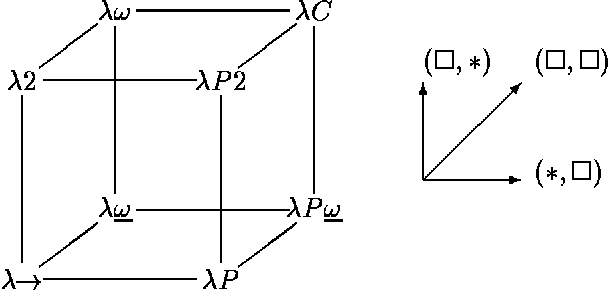
\includegraphics[scale=0.3]{lection-05-cube.png}}
\end{center}
Типовые системы и языки программирования:

Классические и функциональные языки:
\begin{tabular}{lll}
$\lambda_\rightarrow$ & $\{\langle \star,\star \rangle\}$ & Классический Паскаль\\
$\lambda_{\underline{\omega}}$&$\{\langle \star,\star \rangle, \langle \openbox,\star\rangle\}$ & Система F\\
$\lambda_\omega$&$\{\langle \star,\star \rangle, \langle \openbox,\star\rangle, \langle \openbox,\openbox\rangle\}$ & Haskell, Ocaml
\end{tabular}

\vspace{0.3cm}
Языки с зависимыми типами данных (обычно около $\lambda C$):\\
Idris, Coq, Agda, Arend, C++ :).
\end{frame}

\begin{frame}{Изоморфизм Карри-Ховарда}

Рассмотрим формулу с квантором: $\forall x.\pi$.
Ей соответствует $\Pi x.\pi$, а доказательство было бы $\lambda x.P : \Pi x.\pi$. Подробнее:

\begin{center}\begin{tabular}{ll}
$\lambda x^\star.P : \Pi x^\star.\pi : \star$ & $x \in V$, для логики 2 порядка\\
$\lambda x^\upsilon.P : \Pi x^\upsilon.\pi : \star,\text{ если }\upsilon:\star$ & $x \in U\subseteq D$, для (многосортной) логики 1 порядка
\end{tabular}\end{center}

В самом деле: $\forall x.\pi$ требует $\pi[x := \theta]$ при всех $\theta$ (соответствующих $\upsilon$). 
Доказательство: функция $\lambda x.P$, отображающая $\theta$ в терм, обитающий в $\Pi x.\pi$.

%Рассмотрим другие конструкции:

\begin{center}\begin{tabular}{lll}
Логика & $\lambda$-исчисление & Комментарий \\\hline
$\pi$ & $x : \pi$ & Утверждение\\
$\pi(x)$ & $P : \pi(x)$ & Предикат\\
$\forall x\in U.\pi$ & $\lambda x^\upsilon.P : \Pi x^\upsilon.\pi$ & Тотальная функция\\
$\exists x\in U.\varepsilon$ & $ (X, U[x:=X]) : \Sigma x^\upsilon.\varepsilon$ & Зависимая пара
\end{tabular}\end{center}

\end{frame}

\begin{comment}
\vspace{0.5cm}
\begin{exm}
type 
\end{exm}

\begin{exm}
Покажем, что если $\forall x^\upsilon.\pi(x)$ и $\forall x^\upsilon.\xi(x)$, то 

Пусть $\lambda x^\upsilon.P(x) : \Pi x.\pi(x)$ и $\lambda x^\upsilon.Q(x) : \Pi x^\upsilon.\xi(x)$. Покажем, что 
$\forall x.\pi(x) \& \xi(x)$.
То есть, $\lambda x^\upsilon.\langle P(x), Q(x) \rangle$
\end{exm}
\end{comment}

\begin{frame}[fragile]{Idris: пример языка с зависимыми типами}
\small
\begin{verbatim}
data Nat : Type where
    Z : Nat
    S : Nat -> Nat

data Vect : Nat -> Type -> Type where
   Nil  : Vect Z a
   (::) : a -> Vect k a -> Vect (S k) a

(++) : Vect n a -> Vect m a -> Vect (n + m) a
(++) Nil       ys = ys
(++) (x :: xs) ys = x :: xs ++ ys
\end{verbatim}
\end{frame}

\begin{frame}[fragile]{Зависимые типы: printf на Идрис}
\small
\begin{verbatim}
-- Mukesh Tiwari, https://github.com/mukeshtiwari/Idris/blob/master/Printf.idr
data Format = FInt Format
            | FString Format
            | FOther Char Format
            | FEnd

format : List Char -> Format
format ('%' :: 'd' :: cs ) = FInt ( format cs )
format ('%' :: 's' :: cs ) = FString ( format cs )
format ( c :: cs )         = FOther c ( format cs )
format []                  = FEnd

interpFormat : Format -> Type
interpFormat ( FInt f )     = Int -> interpFormat f
interpFormat ( FString f )  = String -> interpFormat f
interpFormat ( FOther _ f ) = interpFormat f
interpFormat FEnd           = String
\end{verbatim}
\end{frame}

\begin{frame}[fragile]{Printf на Идрис}
\small
\begin{verbatim}
formatString : String -> Format
formatString s = format ( unpack s )

toFunction : ( fmt : Format ) -> String -> interpFormat fmt
toFunction ( FInt f ) a     = \i => toFunction f ( a ++ show i )
toFunction ( FString f ) a  = \s => toFunction f ( a ++ s )
toFunction ( FOther c f ) a = toFunction f ( a ++ singleton c )
toFunction FEnd a           = a 

sprintf : ( s : String ) -> interpFormat ( formatString s )
sprintf s = toFunction ( formatString s ) ""

main : IO ()
main = putStrLn (sprintf "String: %s, integer: %d" "alpha" (10+23))
\end{verbatim}
\end{frame}


\end{document}
